\documentclass{article}
\usepackage{fontspec}
\usepackage{parskip}
\usepackage{amsmath}
\usepackage{graphicx}
\usepackage{caption}
\usepackage{tabularx}
\usepackage{float}
\usepackage{subcaption}
\usepackage[backend=biber, citestyle=numeric, sorting=none]{biblatex}
\addbibresource{sxfst.bib}

\setmainfont{Noto Sans}

\begin{document}
\title{\textbf{Screening Fist}}
\author{James Engleback}
\maketitle
\tableofcontents

\section{Abstract}
\textit{Screening Fist} is a screening operation used to train a machine learning model to predict the likelihood of a given enzyme binding to a given small molecule from sequence.
The model is pre-trained on a large and general dataset of protein and small molecule binding pairs scraped from several online sources before retraining on the screening data.
The screening data is generated in-house with a high-throughput, custom developed Cytochrome P450-small molecule binding assay, with which five P450 BM3 mutants were each screened for binding against 980 drug-like molecules.
\par
The retrained model can be used for virtual screening of new enzyme sequences against a specific target molecule, or to query a single sequence against many prospective small molecule binding partners.
It can also be used to design subsequent rounds of screening based on the expected information gain of an experimental design.

% ----------
\section{Introduction}

\subsection{Engineering Problem and Context}
\subsection{Technologies Used}
\subsubsection{Machine Learning}
\subsubsection{Transfer Learning}

Transfer learning is a phenomenon where a model trained on one task, can be re-trained on a different domain-related task  sample-efficiently compared to an untrained model.
For example an object detection model trained from from images of vehicles can transfer efficiently to identification of cell phenotypes from microscopy images.
This is because some learned features generalize well enough to be useful in other tasks, reducing the number is samples required to reach a baseline performance level.

In the domain of protein sequence-based machine learning, thoroughly pre-trained models are available for generating a neural embedding of a given protein that can improve sample efficiency in downstream learning tasks.
Generally, these models are large attention-based models trained \textit{unsupervised} on a large corpus of protein sequences, like the \textit{TrEMBL} collection of \textit{Uniprot}.
In this case, unsupervised training often entails reconstruction of a distorted or masked protein sequence and is run on hardware far beyond the budget of this project.

\subsubsection{The TAPE Benchmark}

Tasks Assessing Protein Embeddings \textcite{tape2019} is a benchmark for comparing numerical representations of protein sequence (learned or otherwise) on a set of biological learning tasks from different domains of protein science. 
It currently contains five tasks:

\begin{enumerate}
\item \textbf{Secondary Structure Prediction Task:}
\item \textbf{Structural Contact Prediction Task:}
\item \textbf{Remote Homology Detection:}
\item \textbf{Fluorescent Protein Landscape Prediction:}
\item \textbf{Protein Stability Landscape Prediction:}
\end{enumerate}

Tasks 4 and 5 are most applicable to protein engineering, since they involve metric prediction from a set of largely similar protein sequences.
The leader boards for performance on these two tasks as of 5 Jun 2022 are:

\textbf{Fluorescence:}

\begin{table}
	\begin{center}
		\caption{Fluorescence TAPE benchmark leader boards \label{tapefluor}}
		\begin{tabular}{l|p{3cm}|l}
			\textbf{Ranking} & \textbf{Model} & \textbf{Spearman's rho}\\
		\hline 
			 1. & Transformer & 0.68 \\
			 2. & LSTM & 0.67 \\
			 2. & Unirep & 0.67 \\
			 4. & Bepler & 0.33 \\
			 5. & ResNet & 0.21 \\
			 6. & One Hot & 0.14 \\
		\end{tabular}
	\end{center}
\end{table}


\textbf{Stability:}

\begin{table}
	\begin{center}
		\caption{\label{tapestab} Stability TAPE benchmark leader boards }
		\begin{tabular}{l|p{3cm}|l}
			\textbf{Ranking} & \textbf{Model} & \textbf{Spearman's rho}\\
		\hline 
			 1. & Transformer & 0.73 \\
			 1. & Unirep & 0.73 \\
			 1. & ResNet & 0.73 \\
			 4. & LSTM & 0.69 \\
			 5. & Bepler & 0.64 \\
			 6. & One Hot & 0.19 \\
		\end{tabular}
	\end{center}
\end{table}

\textbf{Facebook AI Research - Evolutionary-Scale Modelling}
\subsection{Related Work}
\subsection{Overview of This Work}
% ----------
\section{Methods and Development}
\subsection{Assay Development}

In order to generate a P450 BM3-specific dataset on which a model could be re-trained to make binding likelihood predictions on drug-like molecules, a high throughput P450 binding detection assay was developed.
The assay is based on traditional UV-Visible light spectroscopy-based techniques for detection of P450-ligand binding, miniaturized into a 384 well format. 
It relies heavily on automation and a throughput of 980 compounds per day is demonstrated.

\subsubsection{Aim}

The initial aims of this development work were:

\begin{itemize}
	\item Develop a high throughput P450-ligand binding assay based on established biophysical characterisation techniques.
	\item Develop necessary software for design and analysis of each assay.
	\item Compare the precision and accuracy of the assay to existing techniques.
\end{itemize}

\subsubsection{Basis: UV-Visible Spectroscopy for Monitoring Cytochrome P450-Ligand Binding}

The assay is based on a technique for quantifying P450-ligand interactions based on UV-visible photospectroscopy.
The technique consists of the purified Cytochrome P450 heme domain in question in a neutral buffer at around 5-10 µM in a optically clear cuvette.
Since only the heme-containing domain of the P450 is used, no chemical reactions are expected to take place which removes time-sensitivity from the assay.
\par

The UV-visible light absorbance of the sample is typically measured for all wavelengths between 200 and 800 nm, which for a P450 without a ligand bound in the active site should show a large and defined absorbance peak at around 420 nm.
\par
After an initial absorbance measurement of the ligind-free P450, the compound of interest can be titrated into the sample.
On binding to the ligand, the absorbance profile of the P450 changes such that the absorbance at 420 nm ($A_{420}$) decreases and absorbance at 390 nm ($A_{390}$) increases.
\par
The change in $A_{420}$ and $A_{390}$ in response to change in ligand concentration can be quantified and used to derive metrics that indicate affinity between the ligand and P450 using Michaelis-Menten kinetics models.
\par
The original Michaelis-Menten model of enzyme kinetics states:

$$ v = V_{max} \frac{[S]}{[S] + K_M} $$

where $v$ is the reaction velocity - the rate of an enzymatic reaction. 
$V_{max}$ is the maximum possible $v$ for this particular enzyme-substrate pair, $[S]$ is the concentration of the substrate and $K_M$ is the $[S]$ at which $v = V_{max}$.
\par
$V_{max}$ and $K_M$ are useful metrics for quantifying the binding interaction between enzyme and substrate, where low $K_M$ indicates a tight binding interaction and a high $V_{max}$ indicates a large magnitude of response.

Important assumptions in the Michaelis-Menten model of kinetics are:

\begin{enumerate}
	\item The concentration of enzyme is $< K_d$ 
	\item The rate of reaction is directly proportional to the concentration of the substituents
	\item The reaction is at chemical equilibrium at the time of measurement
	\item The interaction is reversible
\end{enumerate}

A variant of this model is applied to Cytochrome P450 photospectroscopy assays, where the response to a ligand is detectable in the 390-420 nm region.
Ligand binding to a P450 alters the electron environment in the heme, which changes the UV-Visible light absorbance profile.
Specifically, absorbance at 420 nm is reduced and absorbance at 390 nm increases.

In this case, $v$ is substituted for $\Delta A_{390} - \Delta A_{420}$ - the magnitude of the P450 response and $K_M$ is substituted for $K_d$ - the dissociation constant between the enzyme and ligand.
This yields the formula:

$$ Response = \Delta A_{390} - \Delta A_{420} = V_{max} \frac{[S]}{[S] + K_d} $$

An example of this is shown in \textbf{figure \ref{arachadionictitration}}, where the fatty acid arachadionic acid was titrated into a sample of P450 BM3 wild-type.

\begin{figure}
	\caption{\label{arachadionictitration} Response of P450 BM3 to Arachadionic Acid from a titration experiment, from which steady-state Michaelis-Menten kinetics can be derived.}
	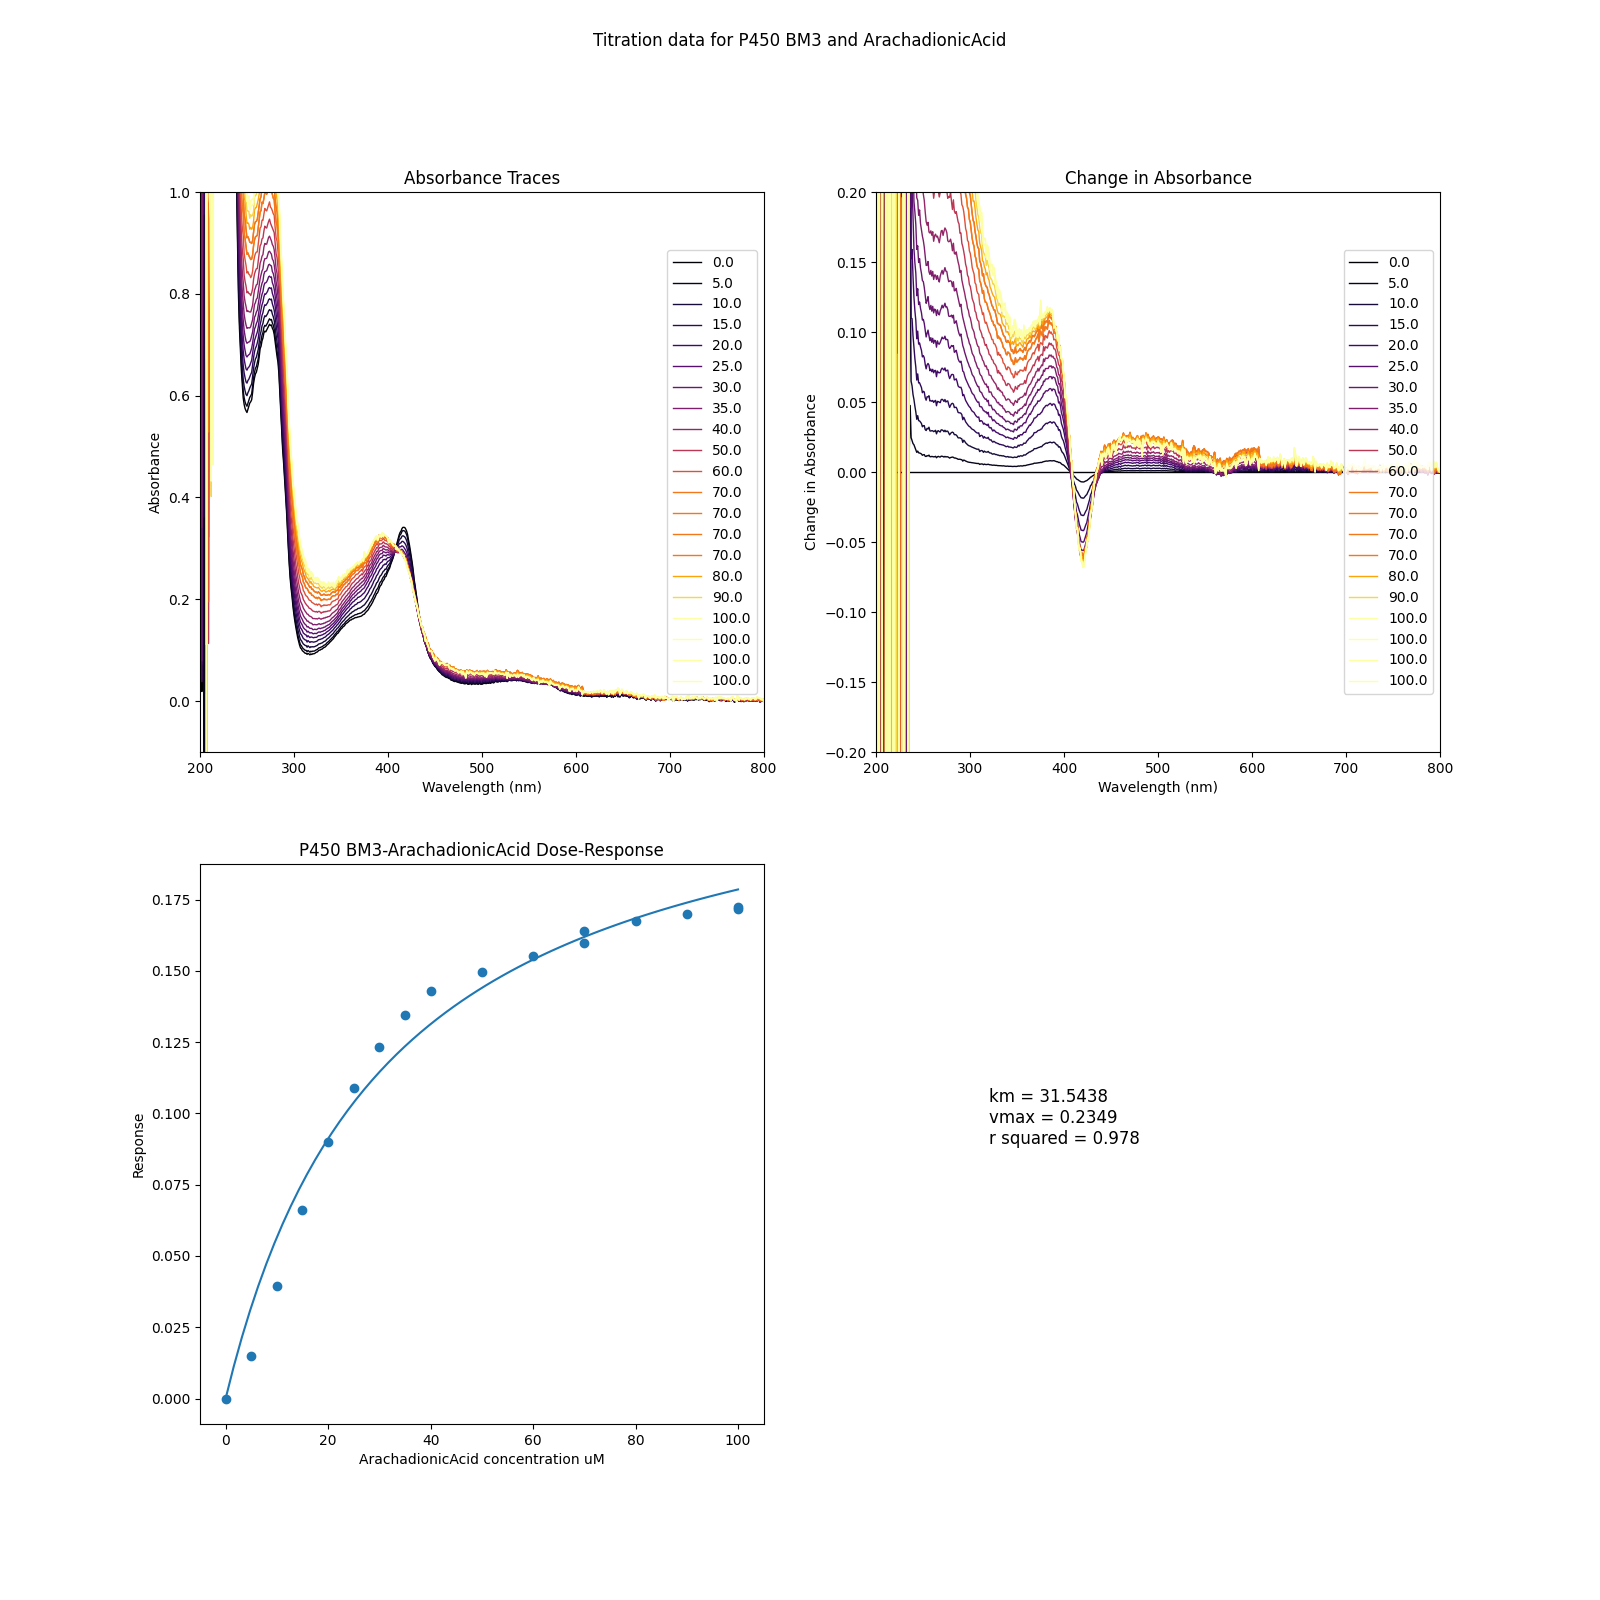
\includegraphics[width = \textwidth]{img/ArachadionicAcid.png}
\end{figure}

% -----------------

\subsubsection{Development}

This style of assay was miniaturized into a 384-well format for the purpose of this project.
The 384-well format permits high throughput screening of compounds for binding with a given P450 provided it is sufficiently stable to last the duration of the experiment without degrading and interfering with measurement.

% echo.py
At micro-scales, precision dispensing of both compound and protein is critical for overall assay precision.
To achieve sufficient precision, compounds were dispensed using an \textit{Echo 550} acoustic liquid handling device, which uses ultrasound to move liquid from a source plate to a destination plate.
In order to achieve the desired dispensing pattern, a custom python package, \texttt{echo}, was developed.
\texttt{echo} facilitates dispensing of compounds in the gradients required by output of a picklist \texttt{csv} file that can be used directly in the \textit{Echo}.
A critical function of this package is that it tracks the volume of compounds in the source plate, which is important in the common case that one compound must be spread over multiple wells.
The package was indispensable in this work.


% ThermodropMulti
During early stages of development, an automated bulk liquid dispensing device - a \textit{ThermodropMulti} was available.
The device uses precise peristaltic pumps to dispense a single liquid into a plate at a single volume very quickly.
Precision in the bulk fluid volume in the plate is helpful in downstream analysis due to the consistent path lengths and concentrations in each well, something that was found to be less consistent when using a multichannel pipette to achieve the same task.
\textbf{Figure \ref{assaydevarachadionic}} shows an example of both the \textit{ThermodropMulti} and \textit{Echo} being used to capture $K_d$ and $V_{max}$ for the binding interaction between P450 BM3 wild-type and arachadionic acid.

\begin{figure}
	\caption{\label{assaydevarachadionic} Michaelis-Menten steady-state kinetics of arachadionic acid and wild-type P450 BM3 captured during assay development.
		 Notably, in this experiment both an \textit{Echo} and \textit{ThermodropMulti} were used in dispensing compound and protein respectively,
		 which accounts for the neatness.
		 The traces were smoothed using a Gaussian kernel to account for noise.}
	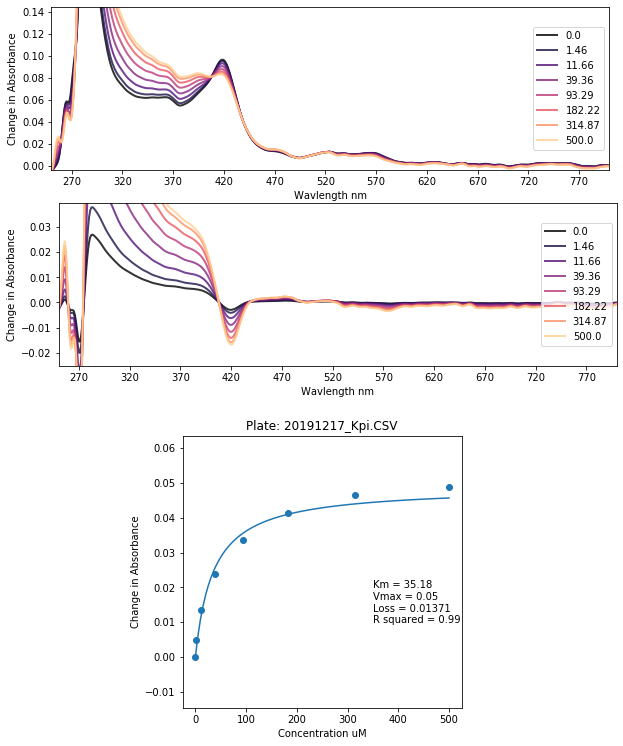
\includegraphics[width = \textwidth]{img/assay-dev-arachadionic.png}
\end{figure}

%%%%% -----------------------
\subsection{Assay Protocol} \label{protocol}

This is a assay protocol for detecting binding interactions between a Cytochrome P450 and multiple small molecule compounds.
The assay has demonstrated scale to a library of 980 compounds and five P450 mutants and with some small adjustments could be improved in scale and precision.

It works in 384 well microplates and uses a microplate reader to capture absorbance profiles from 220-800 nm wavelengths, from which a pattern associated with a P450-small molecule binding interactions can be detected and quantified.  

It was designed for profiling and modelling the effect of mutations on a P450's substrate binding preferences.
This was tested with five P450 mutants against 980 drug-like compounds.
It requires purified P450 protein which limits the rate of data generation, though can scale to more compounds.


\subsubsection{Requirements}

\textbf{Essential:}

\begin{itemize}
\item \textbf{Hardware:}
	\begin{itemize}
	\item \textbf{Microplate reader:} Able to read absorbance for all wavelengths between 220 and 800 nm.
		Used here: \textit{BMG ClarioStar and FluoStar} microplate readers.
	\item \textbf{Labcyte Echo [500 550]:} Acoustic liquid handlers for precise compound dispensing.
\item \textbf{Consumables:}
	In absence of a high precision liquid handling machine, serial dilution of compounds would probably be fine.
	\item \textbf{Enzyme:} A purified Cytochrome P450 - used here were mutants of P450 BM3 at ~800 µM. 
	Note that BM3 is fairly stable at room temperature which facilitates queuing large batches of plates to the plate reader.
	You could run the assay at a low temperature if you use a solvent other than DMSO, which freezes at 19ºC, which interferes with measurement.
	\item \textbf{Compound Library:} A large number of compounds in solvent (e.g. DMSO) in a microplate format.
	Used here was a 980 compound library, dissolved at 10 mM in DMSO in 96 well format.
	\item \textbf{Buffer:} must be optically clear the protein must be stable in it.
	Must not contain potential ligands.
	Used here was 100 mM Potassium Phosphate at pH 7.0 - chosen based on traditional wisdom.
	\item \textbf{384 well microplates - clear bottom:}
	Assay plates with at least 30 µl working volume. 
	Some treated surfaces may be more suitable for unstable proteins.
	Ideally have minimal absorbance in the 390-420 nm region, but this can be corrected for with controls.
			Used here: \textit{ThermoFisher Nunc 384 Well Plates}
			- \textbf{384 well \textit{Labcyte Echo} source plates:} for dispensing compounds to assay plates. 
			Used here were the \textit{Low Dead Volume (LDV)} variety, which have a working volumne of 2.5-12.5 µl, 
			which limits compound waste compared to the standard \textit{Echo} plates (12-65 µl).
	\end{itemize}
\end{itemize}

\textbf{Optional:}
\begin{itemize}
	\item \textbf{Hardware:}
		\begin{itemize}
			\item \textbf{Bulk liquid dispensing:} can be far more accurate than a multichannel pipette when dispensing protein or buffer into wells.
			During development, both a \textit{ThermodropMulti} peristaltic dispenser and a \textit{Hamilton Star} liquid handling robot. 
			Both work well, though use of a bulk liquid dispensing machine is recommended given their speed, lower unit cost and lack of requirement for pipette tips.
			\item \textbf{Microplate reader plate loader:} Autoloading plates into the reader increases throughput capacity significantly.
			I used a \textbf{BMG ClarioStar} plate reader with a stacker module.
		\end{itemize}
	\item \textbf{Consumables:}
		\begin{itemize}
			\item \textbf{BSA:} in assay buffer may have a stabilizing effect on the enzyme - which would improve time stability and reduce errors.
			Time stability is important for scalability.
			\item \textbf{384 well Labcyte Echo DMSO Trays:} for control for DMSO concentration in assay wells by topping up each assay plate to a fixed concentration. 
			Around 5\% is ok with BM3.
		\end{itemize}
\end{itemize}

\subsubsection{Procedure}


\textbf{Summary:}
%\begin{enumerate}
%	\item \textbf{Design \textit{Echo} picklists}
%	\item \textbf{Dispense compounds into \textit{Echo} source plates}
%	\item \textbf{Dispense compounds from \textit{Echo} source plates to empty assay plates}
%	\item \textbf{Stopping point}
%	\item \textbf{Thaw purified P450 and make stock of ~ 10 µM in a neutral buffer, enough for 15.36+ ml per plate (40 µl per well)}
%	\item \textbf{Dispense the diluted protein into the assay plates, centrifuge etc}
%	\item \textbf{Capture UV-Visible light absorbance data between 220 and 800 nm from plates in a microplate reader at room temperature within 3 hours}
%	\item \textbf{Data analysis}
%\end{enumerate}



\begin{enumerate}
% --- 1---- 
	\item \textbf{Design \textit{Echo} picklists:}
	\begin{itemize}
		\item An \textit{Echo} can accept a \texttt{csv} file with column headers: \texttt{Transfer Volume}, \texttt{Volume}, \texttt{Destination Well}, \texttt{Source Well} and optionally: \texttt{Destination Plate Name} and \texttt{Source Plate Name}.
			The Volume must be in nano litres and a multiple of 2.5 and the Source and Destination wells must be in the format \texttt{[A-Z][0-9]+} and exist in the plate layout specified to the \textit{Echo} client at runtime.

		\item The picklist(s) can be generated in a spreadsheet exported to \texttt{.csv} or programmatically.
			Documentation for the \texttt{python} tools used are [documented here.](picklists.md)
	\end{itemize}
% --- 2---- 
\item \textbf{Dispense compounds into \textit{Echo} source plates}
	This can be done with a multichannel pipette, and requires one tip per compound. 
		If the total volume of each compound required is greater than 60 µl then a standard polypropylene \textit{Echo} plate should be used, otherwise a low dead volume plate may be economical
		If not, or for valuable compounds, Low Dead Volume \textit{Echo} may plates should be used.
		These have a working volume of 2.5-12.5 µl, outside of which the \textit{Echo} will refuse to dispense.
	You may need to dispense the same compounds into multiple source wells and the picklists must be designed accordingly.

% --- 3---- 
\item \textbf{Dispense compounds from \textit{Echo} source plates to empty assay plates}
		\begin{enumerate}
			\item Transfer the picklist \texttt{.csv} to the \textit{Echo} host computer.
			\item Launch the \textit{Echo Plate Reformat} client there:
			\item Create New Protocol 
			\item Select Custom Region Definitions
			\item \texttt{File} > \texttt{Import Regions} and select your picklist \texttt{.csv}
			\item \textbf{Optional:} Specify the log output in \texttt{Options}, simulate with \texttt{Run} > \texttt{Simulate} 
			\item Save and run, optionally simulating the run first. 
			Multiple copies of a set of destination plates can be specified if the source plates contain sufficient compound volume.
		\end{enumerate}

% --- 3---- 
	\item \textbf{Stopping point:} Length of pause depends on rate of DMSO evaporation from destination/assay plates and the stability of the compounds at the plate storage conditions. 
		Plates stored in a stack should limit evaporation rate to an extent, though specialised lids for \textit{Echo} plates that limit DMSO evaporation are available.
Up to 24 hours seems ok.
% --- 5---- 

\item \textbf{Thaw purified P450, make stock of ~ 10 µM in a neutral buffer, enough for 15.36+ ml per plate (40 µl per well)}
I heard that thawing fast limits ice crystal formation, which could destroy some protein.
Optionally, in a microcetrifuge, pre-cooled to 4C, spin the protein at 14,000 rpm and carefully transferr to fresh tubes to remove unfolded protein.
	\begin{enumerate}

	\item Measure the stock concentration of the protein in a UV-Vis spectrometer by taking an absorbance trace from 200-800 nm, diluted in the destination buffer.
	There should be a peak at 420 nm, the height of which can be used to calculate the protein concentration with the following equation:

	$$ [P450]  = a e l  $$

       where $a$ is absorbance and $e$ is the extiction coefficient - 95 for P450 BM3 heme domain.
       $l$ is the path length in cm and for the cuvettes used was 1.
       Use the measured stock concentration of P450 to create a working stock of around 10 µM.
       10µM was chosen because it yeilds a reasonably strong signal when in plates.
       Varying the protein concentration doesn't have a big effect on measurements, so err towards using more.


	\item Dilute in neutral buffer to the target working concentration.
	Filtration through a 22 µm syringe filter can remove some precipitates.
	Vacuum filtration can work too but in practice, the protein can pick up binding partners from the filtration equipment contaminants, which can ruin downstream measurements.
	\end{enumerate}

%!!! Warning
%	**Mixed Spin protein:** if the P450 is bound to a substrate it can squash the absorbance peak at 420 nm and raise a peak at 390 nm. 
%	This was an issue with BM3 mutants A82F and A82F/F87V which are particularly promiscuous.
%
%	![mixed spin spec]()
%
%	In this case, the substrate can be removed from the binding site using a column of a lipophilic resin, I used Lipidex 1000.
%	The resin is stored in methanol so it must be washed thoroughly with deionised water before equilibrating with the assay buffer.
%	Adding a salt-based buffer while methanol is still present can cause precipitation and block the column.
%
%	The thawed, mixed-spin P450 is added to the column and left at 4ºC for one hour.
%	It's advisable to create fresh stocks of assay buffer at this point, since it's possible that a buffer contaminant is the result of the mixed spin.
%	Then the protein is flushed from the column with more assay buffer into a clean bijoux and kept on ice.
%	Measure the light absorbance between 200 and 800 nm.
%	If the procedure was successful then the absorbance peak at 390 nm should have subsided and the peak at 420 nm should be high and useable for calculating the protein concentration.

\item \textbf{Dispense the diluted protein into the assay plates, centrifuge}

	An electric multichannel pipette works but accuracy is more limited than with automated dispensing. 
	38 µl of protein working stock needs to be dispensed into each well, which brings the total well volume to 40 µl in cases where the volume of compounds in DMSO in each well is 2 ul.
	If the volume of DMSO in destination wells is not a constant 2 ul, then default to 38 µl of the protein stock.
	The variation in total volume can be corrected for in compound concentration calculations, though the path lenght will vary which affects precision.

	Better than that is a precise bulk liquid handling device.
	I used a \textit{ThermodropMulti} for a while which was fast and accurate.
	Occasionally a nozzle would become blocked either with DMSO ice or precipitates, though the protein still dispensed into the correct well.
	Blockages can be cleared by disassembling the pump head, coupling a syringe of water to the nozzle and flushing.

	It may be necessary to dispense some control plates, with everything but protein.
	This is useful to correct for the intrinsic absorbance of the plate and buffer, as well as the compounds themselves which sometimes have absorbance at the measurement wavelengths.
	A control set of plates for every protein screen may be unnecessary and expensive. 
	One good one should be ok.

	Centrifuge the plates for 2-5 mins at around 2000 rpm to push the well contents to the bottom.
	This step can also ensure that meniscuses are flat and uniform and remove bubbles.
	If possible, centrifuge at room temperature to avoid DMSO ice formation.

\item \textbf{Capture UV-Visible light absorbance data between 220 and 800 nm from plates in a microplate reader at room temperature within 3 hours:}

	The protein is fairly stable over the course of 3 hours.
	On a BMG platereader, measurements take about 15 minutes per plate including the data transfer from device to host machine.
	Using an automated plate loader is recommended, for example a BMG Stacker module.
	In that case, put an empty or waste plate on the top of the stack to limit evaporation from the top assay plate.
	The BMG ClarioStar can be instructed not to read the last plate.

	The stacker occasionally jams due to a solenoid error, which can be due to a misaligned stack of plates.
	It is advisable to un-stack and re-stack the plates using the stacker to check for this kind of issue prior to measurement.

\item \textbf{Data analysis overview}
   More info [here](data.md).
   \begin{enumerate}
	   \item Export the plate measurement data to a workable format, like \texttt{.csv}. 
	   In the BMG Mars software, the operation is simple but on all host machines I've tried it on have been unreasonably slow to open the data files prior to export.
   \item Index the files to their experiments. 
	   I used a \texttt{config.yml} file to track this.
   \item \textbf{Analysis}
		\begin{enumerate}
		\item Match compounds to plate well data.
		\item Match the \textit{Echo} exceptions report to wells to find the actual compound volume in each well.
		\item From each trace, subtract its own absorbance $A_{800}$ at 800 nm.
		   This accounts for baseline drift which can be caused by light scattering from precipitates.
		\item If correcting for compound absorbance with control plates, then subtract the absorbance of each test well from each control well.
		        If the actual compound volumes of the test and control don't match up, it can be an issue if the compound interferes with the absorbance in the 390-420 nm region.
		        If the compound absorbance changes predictably then it can be interpolated.
		\item Curves can be smoothed with Gaussian smoothing using \texttt{scipy.ndimage.gaussian\_filter1d} if necessary.
		        Sources of a jagged curve can be precipitates, which can interfere with downstream analysis.
		\item At this point, changes in the P450 absorbance trace can be identified.
		   Common categories of trace are:
			\begin{itemize}
			   \item Clean absorbance trace, no shift.
			   \item Clean absorbance trace, peak shift from 420 to 390 nm.
			   \item Clean absorbance trace, peak shift from 420 to 424 nm.
			   \item Compound interference in absorbance trace.
			   \item Light scattering in absorbance trace.
			\end{itemize}
		   \item For clean traces with a peak shift from 420 to 390 or 424 nm, biding response can be calculated using the $|\Delta A{390}| - |\Delta A_{420}|$ or $|\Delta A{420}| - |\Delta A_{420}|$  for each compound concentration.
		   With a set of concentration-response data points, the binding dissociation constant $K_d$ can be calculated using the Michaelis-Menten equation for enzyme kinetics:

		   $$ Response = \frac{V_{max} \times [S]}{K_{d} + [S]}$$
		   $$ Response = |\Delta A_{390}| - |\Delta A_{420}| $$

		   Where $[S]$ is a given substrate concentration and $V_{max}$ is the maximum response magnitude possible from the P450 being tested from this compound.
				The metrics $K_d$ and $V_{max}$ can be derived by fitting $|\Delta A{390}| - |\Delta A_{420}|= \frac{V_{max} \times [S]}{K_{d} + [S]}$ can be fit to the P450 substrate concentration-response  data points using a curve fit algorithm like \texttt{scipy.optimize.curve\_fit}.

		   Useful additional metrics for each compound are $R^2$ score of the curve fit, a data quality metric. 

		   An ideal end output of this analysis as a table of compounds, P450s and a qualification or quantification of their binding interactions.

		   Documentation on how I implemented this is [here](data.md)
		\end{enumerate}
   \end{enumerate}
\end{enumerate}

\subsection{Enzyme Production}

\subsubsection{Summary}

This page contains the methods for producing the enzymes used in this screening program.
The enzymes are variants of the Cytochrome P450 BM3:

\begin{table}
	\begin{center}
		\caption{\label{bm3_table} BM3 mutants used in screening}
		\begin{tabular}{l|p{3cm}|l}
		\textbf{ID} & \textbf{Mutations} & \textbf{PDB} \\
		\hline 
		WT   &           & 1BU7 \\
		A82F &   A82F    & 4KEW \\
		DM   & A82F/F87V & 4KEY \\
		1YQO &   T268A   & 1YQO \\
		1YQP &   T268N   & 1YQP \\
		\end{tabular}
	\end{center}
\end{table}

The page shows the method used to create the mutant BM3 expression plasmid DNA, 
expression of the mutants in \textit{E. coli} and their purification.

\subsubsection{Aims}

\begin{itemize}
	\item Create expression plasmids containing the target mutants from an in-house starting point - \texttt{bm3-wt.gb}.
	\item Sequence the plasmids to confirm they carry the mutations
	\item Express the mutants in \textit{E. coli} using those plasmids.
	\item Purify the mutant protein from the \textit{E. coli} harvest.
\end{itemize}


\subsubsection{DNA}

\subsubsection{Starting Material}

An heirloom BM3 Wild-type (heme domain) expression plasmid, [bm3-wt.gb](), 
was inherited and used as the basis for DNA work in this project.
The plasmid is a \textbf{?} pET15(?) expression vector where the BM3 gene has a 6xHis purification tag at the N-terminus,
flanked by a T7 promoter and terminator which leads to high yields in strains of \textit{E. coli} containing the T7 RNA polymerase.
The plasmid also encodes ampicillin resistance and a ? replication origin which leads to a low copy number.


\subsubsection{Primer design and Acquisition}

Mutations were introduced to the wild-type sequence via Polymerase Chain Reaction (PCR)-based site-directed mutagenesis.
Two methods were considered for this task based on commercially available kits, where each imposes different constraints on primer design.
Efforts were made to automate primer design as far as possible with scalability in mind.

The PCR kits used were:

\begin{enumerate}
	\item \textit{New England Biolabs (NEB) Q5 mutagenesis kit} - which requires that primers facilitate cloning of a linear DNA strand from the circular template plasmid and mutation payloads are carried in the tail of one primer.
	The kit includes a cocktail of the DNAse \textit{DPN1}, which disassembles template plasmid methylated in \textit{E. coli} and a kinase and ligase that work to join the ends of the linear DNA into a circular plasmid.
	The reaction is restricted to one payload.

	\item \textit{Agilent Quickchange mutagenesis kit} - which requires a pair of overlapping primers that carry the mutation payload in the mid-section.
	This cloning method produces circular DNA carrying the targeted changes. 
	It has the advantage of allowing multiple payloads carried by multiple primer sets.
\end{enumerate}

Two important considerations based on the template sequence are:

\begin{enumerate}
	\item Adenine-Thymine (AT) richness of the template sequence. Compared to cytosine and guanine (C and G), A and T bind to their complimentary bases weakly.
		This results in weak primer binding to the template sequence, measurable by a low primer \textit{melting temperature} $T_m$.
	To compensate, primers must be longer than they otherwise would be for a sequence richer in CG, which increases their cost and their chance of self-binding.
	The template sequence used here is AT-rich - at $x\%$
	\item Repetitions and palindromic regions of the template sequence. 
		If the sequence surrounding a mutation target area contains these features, then the likelihood of \textit{mis-priming} by binding to an off-target sequence area is high, so too is the likelihood of a non-functional, self-binding primer.
\end{enumerate}


\subsubsection{PCR and Work Up}




\subsubsection{Sequencing}

Purified plasmid DNA ostensibly conataining the target mutations, having been harvested and purified from DH5a \textit{E. coli} cells, was shipped to \textit{Eurofins Genomics} for sequencing using their \textit{TubeSeq} service, which uses a variant of Sanger Sequencing.
Sequencing primers for this matched the T7 promoter and terminator and provided coverage of the targetted region.


\subsection{Expression}

Having been sequenced and confirmed to carry the target mutations, the mutant plasmids were used to produce the mutant protein \textit{en masse} via a \textit{BL21 DE3 E. coli} strain, which contains a T7 RNA polymerase under the control of a \textit{lac} promoter.

\subsubsection{Materials}

\begin{itemize}
	\item Expression plasmid encoding mutant P450 BM3
	\item \textit{BL21 DE3 E. coli} - NEB. This domesticated \textit{E.coli} strain is shipped in a transformation buffer.
	\item Auto-induction \textit{Terrific Broth} (TB) media, which contains glucose and a lactose analog. 
	The lactose analog triggers expression of T7 RNA-polymerase in \textit{BL21 DE3 E. coli} and the subsequent expression of the target protein between the T7 promoter and terminator regions. 
	The glucose inhibits this until it is consumed by the cells, which allows them to multiply to sufficient numbers before diverting energy to production of the target protein.
	\item Ampicillin - the antibiotic for which resistance is encoded in the target plasmid, ensuring that all cells in the growth media contain this resistance.
	Assuming no ampicillin-resistant contaminants, all cells should be \textit{BL21 DE3 E. coli} containing the target plasmid.
	\item $\Delta$ Amino-Levulnic acid ($\Delta$-ALA) - a precursor to heme, ensuring heme availability for the large amount of BM3.
\end{itemize}

\subsubsection{Method}

\subsubsection{Purification}

\subsection{Screening}

Throughput the screening process, the protocol described in section \ref{protocol} was employed.
Six concentrations of each target compound were dispensed with the aim of determination of the $V_{max}$ and $K_d$: 0.0, 5.26, 55.61, 156.72, 306.74 and 500 µM.
These values were generated from six linearly spaced values between 0 and 1 squared, then scaled to the starting concentration and final volume.
This method saved some compound compared to a straightforward linear spacing of values between 0 and 500 µM - the maximum concentration possible given a 10 mM starting stock in DMSO without exceeding a total of 5\% v/v solvent.
\par
During the first run, control experiments where compounds were present in buffer only were included for downstream correction of the compounds inherent UV-Visible light absorbance, though it was thought to be unnecessary to repeat this for each subsequent screen, since it is wasteful of resources, particularly the compounds themselves.

Each of the five enzymes was screened against all 980 compounds over the course of a day each.



% -------------------------------

\subsection{Model Design and Construction}

The model aims to predict the binding likelihood between a given protein sequence and chemical structure, illustrated in equation \ref{pbinding}.

$$
\label{pbinding}
P_{binding} = fn(sequence, smiles)
$$

This page describes the deep learning model constructed for this project.
The model is designed to estimate the likelihood of a binding interaction between a given Cytochrome P450 sequence and a ligand SMILES code.
The intended end uses of the model are:

1. Virtually screening sequences for potential activity with a given compound.
2. Optimally design an enzyme-ligand screening experiment.


\subsubsection{Approach: Recommender Systems}

Abstractly, the problem of predicting the binding likelihood between a one of $m$ proteins and one of $n$ small molecules can be likened to filling empty the values of an $n \times m$ matrix, where rows and columns refer to proteins and small molecules and values are the probability of a binding interaction between the two:

\begin{center}
$
\begin{matrix} 
	 & compound_i & compound_{i+1} & ... & compound_{i+n} \\
	sequence_i  & P_{binding_{i,j}} &  &  & \\  
	sequence_{i+1} &  &  &  &  \\
	 \vdots &  &  & \ddots &  \\
	sequence_{i+m} &  &  &  &   \\
\end{matrix}
$
\end{center}

Some $P_{binding}$ values are known, which in the perspective of $n \times m$ possible values where $n$ and $m$ approach infinity, coverage is sparse.

This type of problem has been addressed in recommender systems, which in the context of streaming services translates to a matrix of $n$ users and $m$ paces of content.
Known values are likes and engagement metrics and are similarly sparse, and blanks can be filled with the probability of a successful recommendation.

Machine learning models can be trained to predict the unknown values based on a numerical representation of the user and content.
The prediction can be cast as a classification problem.
To overcome the lack of negative data points, presumed negative data can be generated by sampling a random user: content pair, which should be treated with caution.

In this work, a machine learning model classifies pairs of protein sequence and small molecules as binding or not.
Negative samples are generated by randomly sampling a sequence and small molecule, which given the vastness of sequence and chemical space may be reasonable in a large number of cases, though this assumption is treated with caution.
A Binary Cross Entropy loss function is employed here where true positives and synthesized negatives are weighted evenly.

\subsubsection{Data}

Small molecules are represented as SMILES codes in the dataset, which are parsed using \texttt{rdkit} and then into 2048 bit fingerprint vectors using the \texttt{RdkitFingerprint}.
Molecular fingerprints are generated by hashing functions based on an input molecule such that similar molecules are assigned similar fingerprints, which makes them useful in featurizing small molecules for machine learning tasks.
The fingerprints are represented as a $b \times 2048$ tensor where $b$ is batch size.

Sequences are represented in the dataset as strings where each character $c_i$ is a single letter amino acid code:

$$c_i \subset{ACDEFGHIKLMNPQRSTVWY}$$

Roughly, characters are encoded as tensors of the integers that index their position in the list $\begin{matrix} ACDEFGHIKLMNPQRSTVWY\end{matrix}$, with extra positions to represent null values, start of frame and end of frame characters.

	\subsubsection{Pre-Training Data}

\subsubsection{Training Data}

\subsubsection{Model Architecture}

Given the model aims to predict:
$$
P_{binding} = fn(sequence, smiles)
$$

A neural network was devised to generate a prediction of $P_{binding}$ from an input of a protein sequence and a chemical SMILES code.
The network can be split into three parts:

\begin{itemize}
	\item \textbf{Sequence Embedding:} For a given protein $sequence$, output a tensor encoding a neural embedding $z_{sequence}$.
	\item \textbf{Chemical Embedding:} For a given chemical $smiles$ encoding, outputs an embedding $z_{smiles}$.
	\item \textbf{Prediction Head:} For the embeddings $z_{smiles}$ and $z_{sequence}$, output a prediction $P_{binding}$.
\end{itemize}

The architecture is illustrated in \ref{modelarch}.

\begin{figure}
	\begin{center}
	\caption{\label{modelarch} Architecture of the model constructed for this project}
	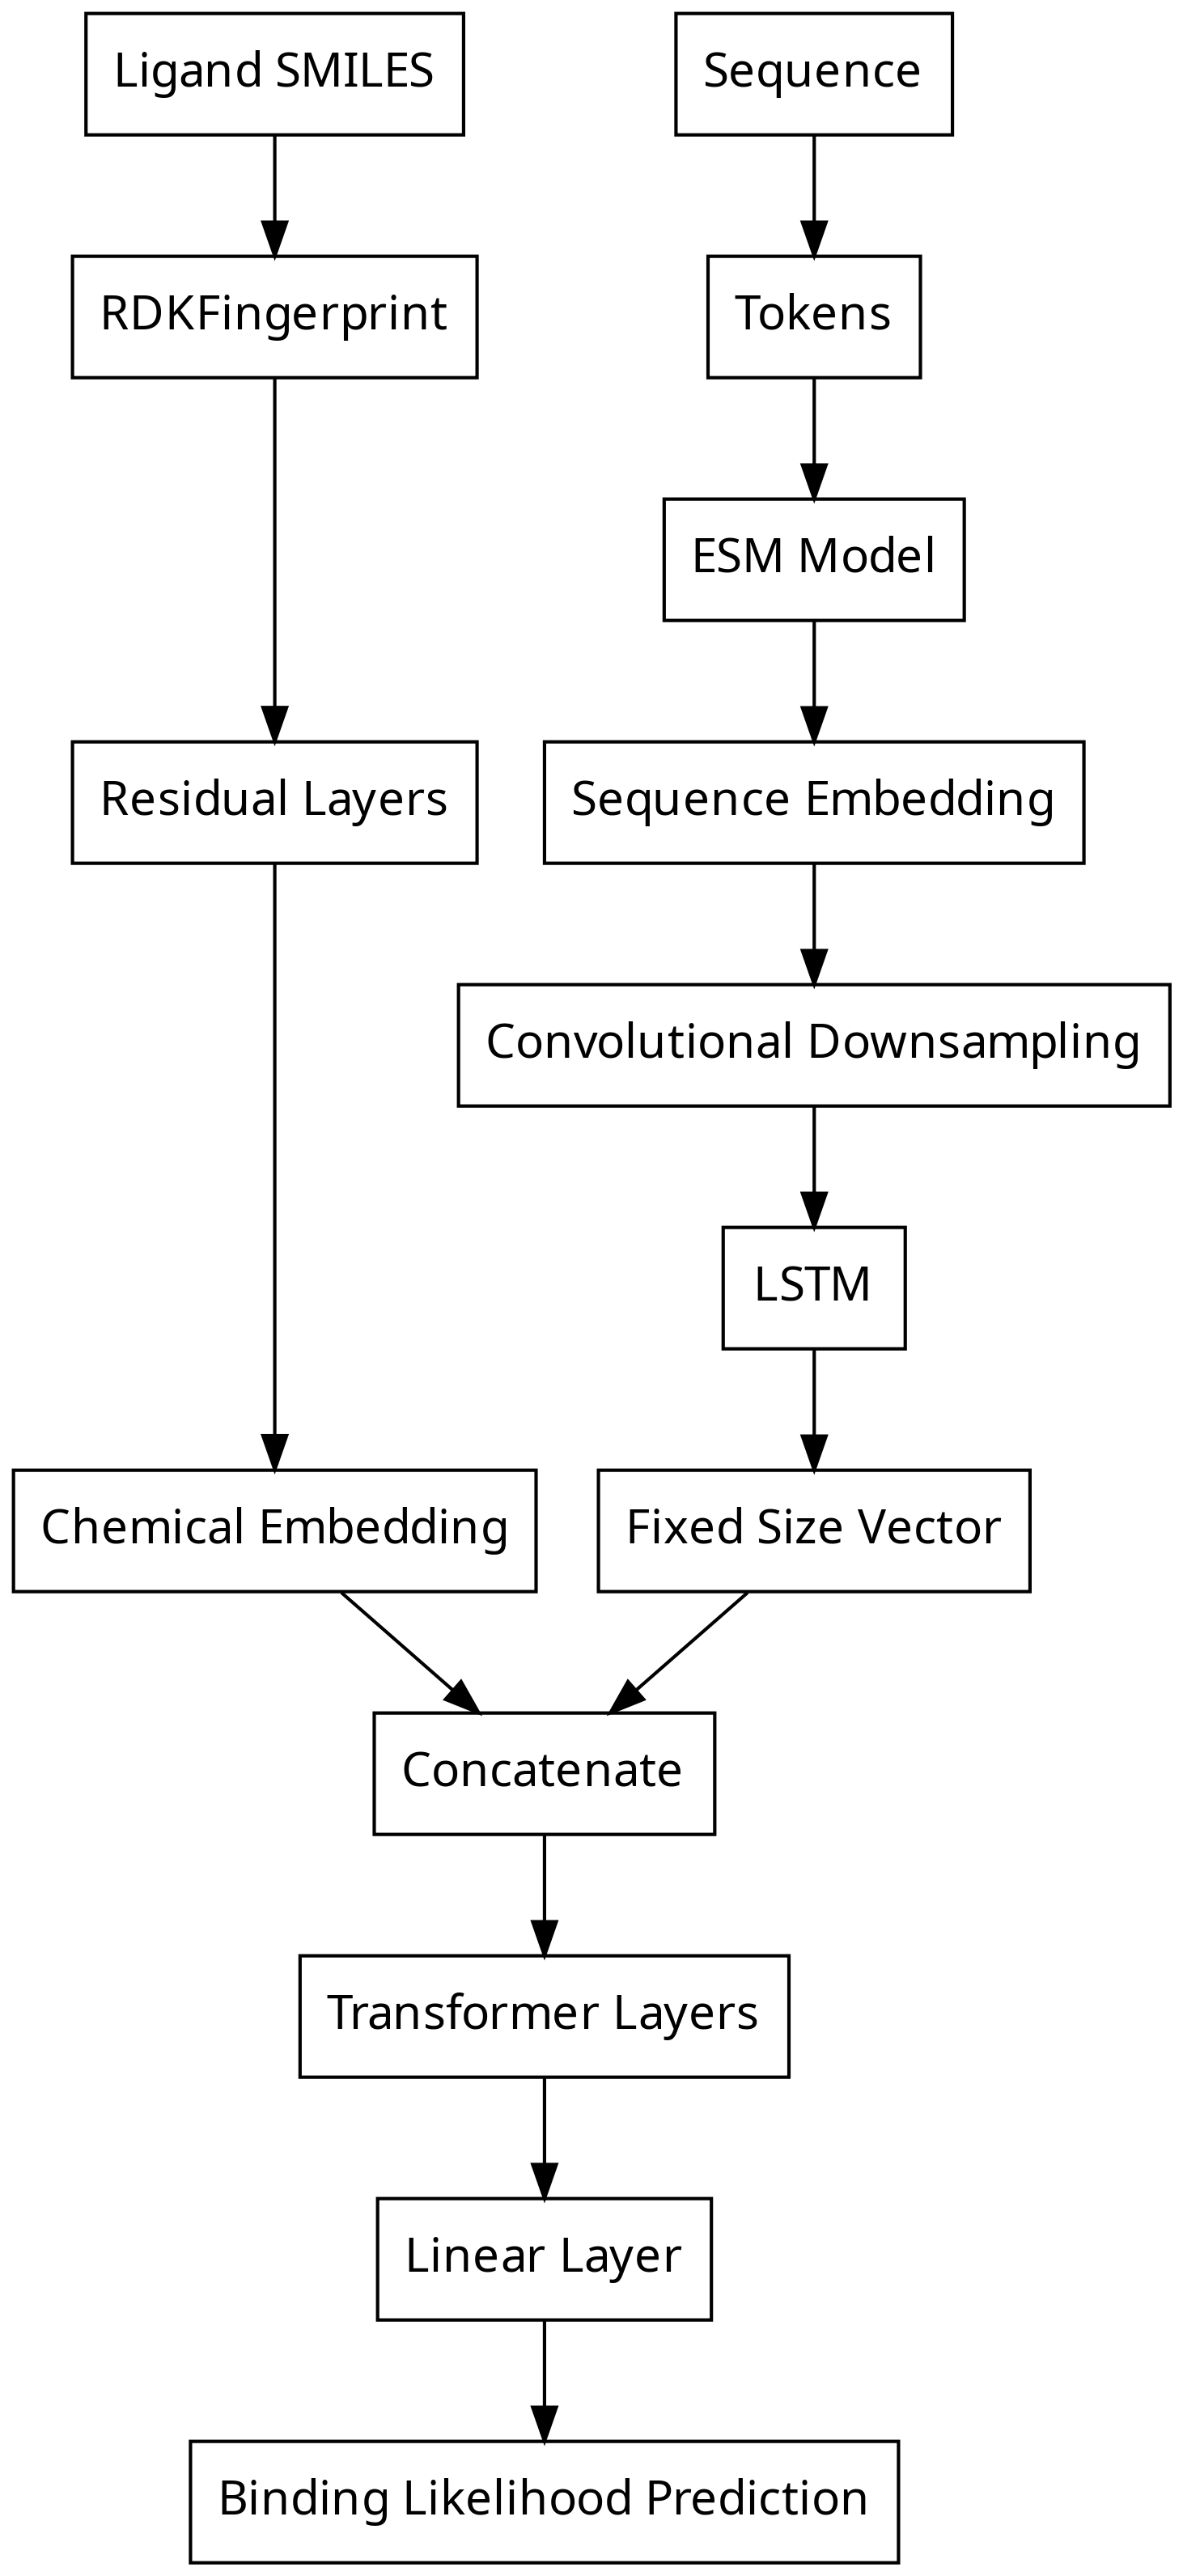
\includegraphics[height=0.8\textheight]{img/model.png}
	\end{center}
\end{figure}

\subsubsection{Sequence Embedding}

%Sequences were embedded using the pre-trained \texttt{esm1_t6_4equation 3M_UR50S} model \textcite{rives2021biological}, which receives an input of a tokenized protein sequence and outputs a tensor of size $b l d$ where $b$ is batch size, $l$ is sequence length and $d$ is 35.

Although this model is the smallest of the ESM collection, on the single \textit{NVIDIA Quadro RTX 6000} used it still occupied most of the 24 GB of available memory and most of the processing capability, which lead to long training times and difficulty in training more than one model in parallel on the same machine.

This could be remedied, however since in the complete \texttt{o3f.csv} dataset and the screening dataset there are 2947 unique sequences, so it was economical to pre-compute the embeddings and save them to disk.
This resulted in a roughly 4$\times$ speedup in training time and massively reduced the memory requirements, allowing several models to be trained in parallel on a single GPU.
This also saved costs significantly.

\subsubsection{Chemical Embedding}

As mentioned, chemical SMILES were hashed into chemical fingerprints using the \texttt{rdkit} \texttt{RDKFingerprint} method as a means of representation, yielding a 2048-bit vector for each compoundagainThe vectors were converted to tensors and served as an input to a residual neural network that output an embedding that would later be used to form a combined representation of both compound and sequence for binding likelihood prediction.

\subsubsection{Prediction Head}

The combined sequence and compound embeddings served as input to the prediction head, which output a single number that indicated a binding likelihood prediction for the two inputs.

Both residual neural networks and transformers were compared as prediction head architectures.
Each consisted of 2-6 stacked layers of either residual or transformer layers with a fixed hidden layer size for convenience of automated assembly.
The final layer in both cases was a single linear layer with a single output and a sigmoid function to output a number between 0 and 1 representing binding probability.

\subsubsection{Pre-Training, Training and Evaluation}

Training was done in two stages, each with a performance evaluation, during which several models with varying architectures and hyper-parameters were trained and compared.
All training was done on a \textit{Linode} \texttt{g1-gpu-rtx6000-1} which cost \$1.50 per hour and was equipped with the following hardware specifications:

\begin{table}
	\begin{center}
		\caption{\label{bm3_table} BM3 mutants used in screening}
		\begin{tabular}{l|p{3cm}|l|l}
			\textbf{Item} & \textbf{Specifications} & \textbf{Number}  & \textbf{Size}\\
		\hline 
		CPU  & Intel(R) Xeon(R) Gold 6148 CPU @ 2.40GHz & 8 \\
		RAM  & ?  & N/A & 30 GB \\
		Disk & ?  & 1   & 630 GB \\
		GPU  & NVIDIA Quadro RTX 6000 & 1 & 20 GB VRAM \\ 

	\end{tabular}
	\end{center}
\end{table}

\begin{enumerate}
	\item \textbf{Pre-Training:} This was done with the larger, more general \texttt{o3f} dataset, which was randomly split into training and validation partitions, the latter of which was used sparingly to avoid model bias.
	Pre-training lasted up to 64 epochs with a batch size up to 64.
	For each sample, a random sequence and SMILES pair were sampled as a presumed negative sample.
	The loss function used was binary cross entropy used with an Adam (Adaptive momentum) optimizer.
		Loss was tracked live using the \textit{Weights and Biases} API which was useful to evaluate models as they trained and terminate them where necessary.
	Model weights were saved in each epoch and after training the model was evaluated for precision and accuracy on a subset of the training data.
	The metrics gathered were: 

		\begin{enumerate}
			\item Mean binary cross entropy loss over evaluation.
			\item Mean precision
			\item A confusion matrix
			\item A receiver operator curve (ROC)
			\item A precision recall curve
			\item A detection error trade-off (DET) curve
		\end{enumerate}

	\item \textbf{Training:} This was done with the manually annotated screening dataset.
	An issue with the data was the class imbalance in that there were very few positive examples relative to negative.
		This was addressed by using \textit{Synthetic Minority Oversampling} (SMOTE) whereby the rarer positive data were re-sampled until they number that of the negative data.
	The total size of the re-sampled data was 6666 points, which were then split 3:1 into training and validation sets of size 4999 and 1667 respectively.
		A model pre-trained on the larger \texttt{o3f} dataset was re-trained on this set and evaluated for performance in the same manner as with the \texttt{o3f} data, visualised in the following section.
\end{enumerate}

\subsubsection{Evaluation}

%## Sequence Optimization
%
%## Active Learning


% ----------
\section{Results}
\subsection{Screening Data Analysis}

The data gathered for the screening experiments was saved in the \texttt{git} repository  \texttt{https://github.com/jamesengleback/screening-fist} in the \texttt{lab} directory.
Within the \texttt{lab} directory are directories for each screening experiment.
These include a \texttt{config.yml} file which maps data files to experiments for analysis.
\par
The script \texttt{sxfst/scripts/data\_proc2.py} was used to process the data into a large \texttt{csv} file containing each raw trace and its metadata.
By consolidating the data into a single file, fewer time-consuming operating system calls are made in downstream analysis which decreases the time cost of those tasks.

The script attempted to use the \textit{Echo} logs from each run to calculate the actual volume of each compound dispensed, since towards the end of the screening program shortages of compound made it impossible to fully dispense some experiments.
In retrospective this function did not perform properly, since all experiments are later annotated as having the target volumes of each compound.
This cannot be the case since it was casually observed that some compounds were completely depleted by the end of the screening program.
This issue is significant, leading to false negatives where a lack of response cannot be attributed to either a lack of compound or a true negative response.
This coding issue can be solved, but was not due to time constraints.

The downstream analysis in question was done using the script \texttt{sxfst/scripts/data\_analysis.py} which normalizes the traces, subtracts the control traces from them and calculates the P450 response to each compound, creating a plot in the process.
An example of one such plot is in \textbf{figure \ref{screeninghit}}.

The traditional response calculation method using $\Delta A_{390} - \Delta A_{420}$ proved ineffective for analysis of this data due to the noise, which would often result in scattering that increased the absorbance at the short wavelengths in ways that were occasionally unpredictable.

Instead, the gradient of each trace was taken by convolution of the kernel $\begin{bmatrix} -1 & 0 & 1 \end{bmatrix}$ across the smoothed and normalized traces.
The gradients were invariant to total absorbance, which was often perturbed by what appeared to be light scattering, but achieved a similar effect to calculation of $\Delta A_{390} - \Delta A_{420}$.
From the gradients, response was calculated as $|{\frac{\delta y}{\delta x_{390}}}| + |{\frac{\delta y}{\delta x_{420}}}|$.

Although this proved successful, the automated curve fitting to the response was not, outputting a constant value of 32 µM for each experiment - the lower $K_d$ bound.
With extra development this issue can likely be solved, but in order to keep within time constraints, an alternative solution was implemented.

%% manual annotation

The alternative solution was manual annotation of the plots output by the script.
Though crude, this method did yield a list of ostensible \textit{hits} as well as a list of anomalous results that were to be ignored.

Using this approach, 149 hits of the total 4900 compounds were identified, listed in the file \texttt{lab/hits.txt} in the repository.
These were used to create a \texttt{csv} file containing the full sequence and SMILES code for each enzyme compound pair and a boolean value that was true if that experiment was annotated as a \textit{hit}.
There are several drawbacks to this that should be noted:

\begin{itemize}
	\item \textbf{Human Error:} Although several passes over the data were done, the order was never randomized and there was only one annotator. 
		Since there are 4900 experiments, even if the annotator averages 1 second per annotation the runtime of an annotation run is 81 minutes, which will likely cause fatigue and subsequent errors.
		Since the order was not randomized, fatigue-induced error is more likely to occur in the same regions of the dataset in each pass.
	\item \textbf{False Negatives} due to a lack of properly functional compound concentration calculation, which would yield results that appear negative due to a lack of compound without being properly labelled as such.
		Another source of false negatives is the obfuscation of hits by noise in the traces due to scattering or compound absorbance that in some cases proved hard to correct for.
\end{itemize}

\begin{figure}
	\caption{\label{screeninghit} A good example of a positive result or \textit{hit} between BM3 A82F and \textit{Gestodene}. $K_d$ was calculated as 32 µM, which reflects an issue in the curve fitting rather than the actual $K_d$.}
	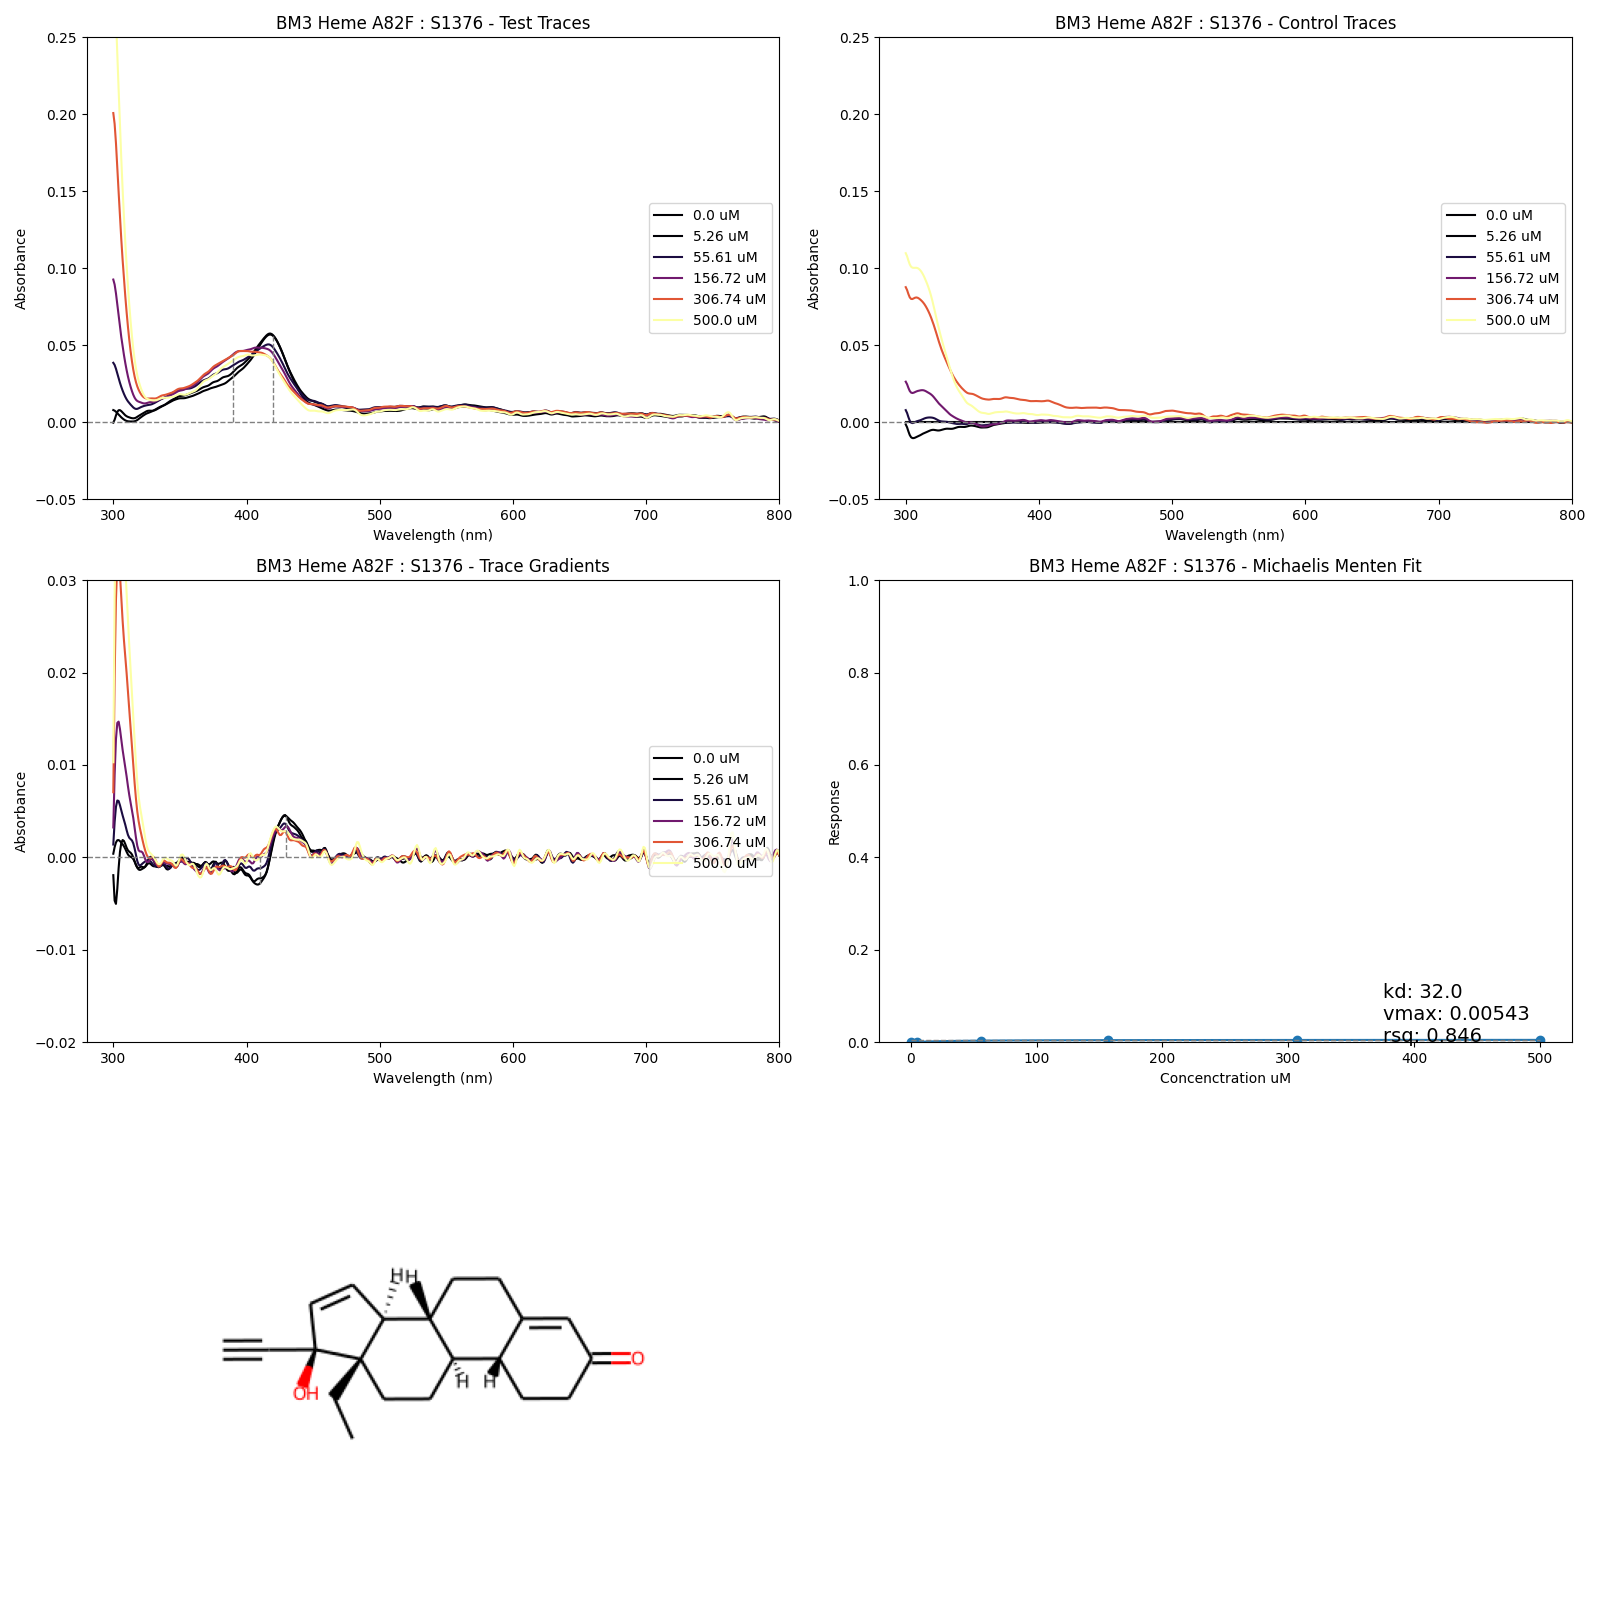
\includegraphics[width = \textwidth]{img/BM3-Heme-A82F:S1376.png}
\end{figure}

\subsection{Model Training}

\subsubsection{Pre-training}

Given constraints on money towards computing resources, a hyper-parameter sweep was not viable.
Instead, a small selection of models were trained and evaluated and the best of those was retrained on the screening data.
Model architecture and hyper-parameters were directly configurable by supply of arguments to the training script \texttt{model/train.py}, from which the best performing model was obtained using the command \texttt{./train.py -i data/o3f.train.csv --transformer --cuda --emb\_size\_head 2560 --n\_layers\_head 3 --emb\_size\_fp 512 --n\_layers\_fp 4 --num\_conv\_layers\_pool 3 --kernel\_size\_pool 9 --stride\_pool 3 --lstm\_hs\_pool 1024 --lr 1e-5 --batch\_size 64 -e 32
}, which is consolidated in \textbf{table \ref{frostybreezeparams}}.

\begin{table}
	\caption{\label{frostybreezeparams} Parameters for the best performing model in pre-training, designated the identifier \textit{frosty-breeze-83} by the \textit{Weights and Biases} API.}
	\begin{center}
	\begin{tabular}{ll}
		\textbf{Parameter} &     \textbf{Value} \\
		\hline
		lr                   &             $10^{-5}$ \\
		esm                  &   esm1\_t6\_43M\_UR50S \\
		cuda                 &                True \\
		load                 &                None \\
		test                 &               False \\
		input                &  data/o3f.train.csv \\
		epochs               &                320 \\
		batch\_size           &                640 \\
		emb\_size\_fp          &               512 \\
		n\_layers\_fp          &                 4 \\
		stride\_pool          &                 3 \\
		transformer          &                True \\
		lstm\_hs\_pool         &              1024 \\
		emb\_size\_head        &              25 \\
		n\_layers\_head        &                 3 \\
		kernel\_size\_pool     &                 9 \\
		num\_conv\_layers\_pool &                 3 \\
		num\_lstm\_layers\_pool &                 2 \\
	\end{tabular}
	\end{center}
\end{table}

%img/frosty-breeze-83-eval.png
%img/frosty-breeze-83-vivid-breeze-91-devout-thunder-90-eval.png
%img/frosty-breeze-83-vivid-breeze-91-eval.png
\begin{figure}
	\caption{\label{frostybreeze} Model evaluation report after pre-training for the model designated \textit{frosty-breeze-83}. Evaluation was on \texttt{o3f.test.csv} - a held-back partition of the pre-training dataset. Depicted are:
	mean binary cross entropy loss the course of training on \texttt{o3f.train.csv},  
	a confusion matrix, 
	a receiver operator curve (ROC), 
	a precision recall curve,
	a detection error trade-off (DET) curve and 
	mean precision and mean binary cross-entropy loss over evaluation.}
	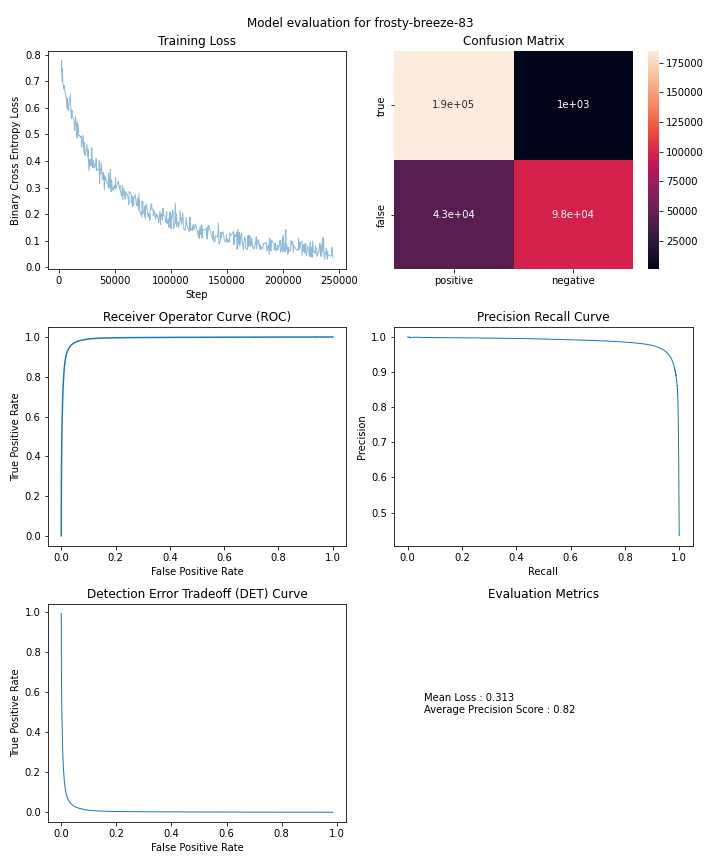
\includegraphics[width = \textwidth]{img/frosty-breeze-83-eval.png}
\end{figure}

\begin{figure}
	\caption{\label{devoutthunder} Model evaluation for another instance of \textit{frosty-breeze-81}, this time designated \textit{devout-thunder-90}, again retrained on the lab-based screening dataset \texttt{screening-data.train.csv} and evaluated on \texttt{screening-data.test.csv}. The report uses the same methods as in figure \ref{frostybreeze}}
	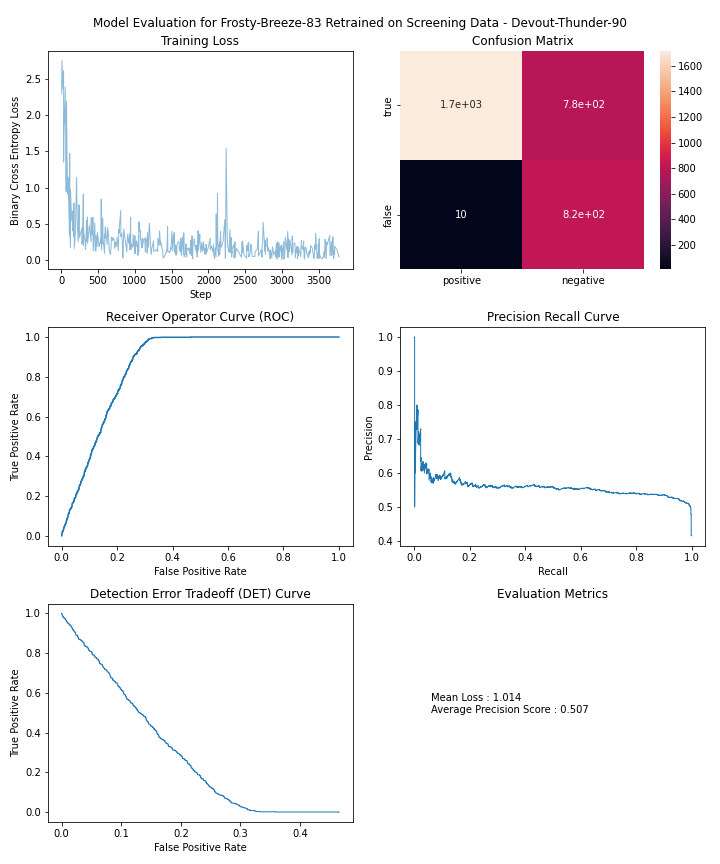
\includegraphics[width = \textwidth]{img/frosty-breeze-83-vivid-breeze-91-devout-thunder-90-eval.png}
\end{figure}
\begin{figure}
	\caption{\label{vividbreeze} Model evaluation report after pre-training for the model designated \textit{vivid-breeze-91}. }
	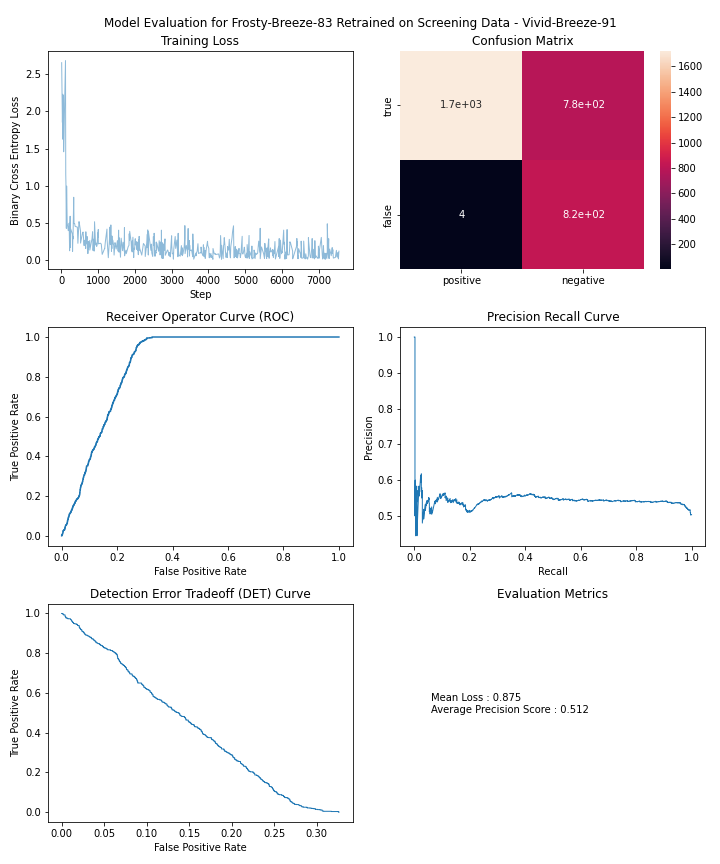
\includegraphics[width = \textwidth]{img/frosty-breeze-83-vivid-breeze-91-eval.png}
\end{figure}
\subsection{Model Application}
% ----------
\section{Discussion and Future Work}

\printbibliography

\end{document}
